%%%%%%%%%%%%%%%%%%%%%%%%%%%%%%%%%%%%%%%%%
%
% CMPT xxx
% Fall 2020
% Lab One
%
%%%%%%%%%%%%%%%%%%%%%%%%%%%%%%%%%%%%%%%%%

%%%%%%%%%%%%%%%%%%%%%%%%%%%%%%%%%%%%%%%%%
% Short Sectioned Assignment
% LaTeX Template
% Version 1.0 (5/5/12)
%
% This template has been downloaded from: http://www.LaTeXTemplates.com
% Original author: % Frits Wenneker (http://www.howtotex.com)
% License: CC BY-NC-SA 3.0 (http://creativecommons.org/licenses/by-nc-sa/3.0/)
% Modified by Alan G. Labouseur  - alan@labouseur.com
%
%%%%%%%%%%%%%%%%%%%%%%%%%%%%%%%%%%%%%%%%%

%----------------------------------------------------------------------------------------
%	PACKAGES AND OTHER DOCUMENT CONFIGURATIONS
%----------------------------------------------------------------------------------------

\documentclass[letterpaper, 10pt,DIV=13]{scrartcl} 

\usepackage[T1]{fontenc} % Use 8-bit encoding that has 256 glyphs
\usepackage[english]{babel} % English language/hyphenation
\usepackage{amsmath,amsfonts,amsthm,xfrac} % Math packages
\usepackage{sectsty} % Allows customizing section commands
\usepackage{graphicx}
\usepackage[lined,linesnumbered,commentsnumbered]{algorithm2e}
\usepackage{listings}
\usepackage{parskip}
\usepackage{lastpage}
\usepackage{hyperref}
\usepackage{tabularx}
\usepackage{graphicx}
\graphicspath{ {./images/} }

\allsectionsfont{\normalfont\scshape} % Make all section titles in default font and small caps.

\usepackage{fancyhdr} % Custom headers and footers
\pagestyle{fancyplain} % Makes all pages in the document conform to the custom headers and footers

\fancyhead{} % No page header - if you want one, create it in the same way as the footers below
\fancyfoot[L]{} % Empty left footer
\fancyfoot[C]{} % Empty center footer
\fancyfoot[R]{page \thepage\ of \pageref{LastPage}} % Page numbering for right footer

\renewcommand{\headrulewidth}{0pt} % Remove header underlines
\renewcommand{\footrulewidth}{0pt} % Remove footer underlines
\setlength{\headheight}{13.6pt} % Customize the height of the header

\numberwithin{equation}{section} % Number equations within sections (i.e. 1.1, 1.2, 2.1, 2.2 instead of 1, 2, 3, 4)
\numberwithin{figure}{section} % Number figures within sections (i.e. 1.1, 1.2, 2.1, 2.2 instead of 1, 2, 3, 4)
\numberwithin{table}{section} % Number tables within sections (i.e. 1.1, 1.2, 2.1, 2.2 instead of 1, 2, 3, 4)

\setlength\parindent{0pt} % Removes all indentation from paragraphs.

\binoppenalty=3000
\relpenalty=3000

%----------------------------------------------------------------------------------------
%	TITLE SECTION
%----------------------------------------------------------------------------------------

\newcommand{\horrule}[1]{\rule{\linewidth}{#1}} % Create horizontal rule command with 1 argument of height

\title{	
   \normalfont \normalsize 
   \textsc{CMPT 424N - Fall 2020 - Dr. Labouseur} \\[10pt] % Header stuff.
   \horrule{0.5pt} \\[0.25cm] 	% Top horizontal rule
   \huge Project Three  \\     	    % Assignment title
   \horrule{0.5pt} \\[0.25cm] 	% Bottom horizontal rule
}

\author{Ryan Sheffler \\ \normalsize Ryan.Sheffler1@Marist.edu}

\date{\normalsize\today} 	% Today's date.

\begin{document}
\maketitle % Print the title

%----------------------------------------------------------------------------------------
%   start PROBLEM ONE
%----------------------------------------------------------------------------------------
\stepcounter{section}
\stepcounter{section}
\stepcounter{section}
\stepcounter{section}
\section{Lab Five}

\subsection{}
Draw four Gantt charts of the processes given on the lab sheet.

\begin{center}
$\begin{tabularx}{\textwidth}{|1|X|X|X|X|X|X|X|X|X|X|X|X|X|X|X|X|X|X|X|}
\hline
Algorithm & 1 & 2 & 3 & 4 & 5 & 6 & 7 & 8 & 9 & 10 & 11 & 12 & 13 & 14 & 15 & 16 & 17 & 18 & 19 \\ 
\hline
 FCFS & P_1 & P_1 & P_1 & P_1 & P_1 & P_1 & P_1 & P_1 & P_1 & P_1 & P_2 & P_3 & P_3 & P_4 & P_5 & P_5 & P_5 & P_5 & P_5 \\ 
\hline
SJF & P_2 & P_4 & P_3 & P_3 & P_5 & P_5 & P_5 & P_5 & P_5 & P_1 & P_1 & P_1 & P_1 & P_1 & P_1 & P_1 & P_1 & P_1 & P_1 \\ 
\hline
NP Priority & P_2 & P_5 & P_5 & P_5 & P_5 & P_5 & P_1 & P_1 & P_1 & P_1 & P_1 & P_1 & P_1 & P_1 & P_1 & P_1 & P_3 & P_3 & P_4 \\ 
\hline
Round Robin & P_1 & P_2 & P_3 & P_4 & P_5 & P_1 & P_3 & P_5 & P_1 & P_5 & P_1 & P_5 & P_1 & P_5 & P_1 & P_1 & P_1 & P_1 & P_1 \\ 
\hline
\end{tabularx}$
\end{center}

\subsection{}
What is the turnaround time for each process with each algorithm?

\begin{center}
\begin{tabularx}{\textwidth}{|X|X|X|X|X|}
\hline
& FCFS & SJF & NP Prio & RR \\
\hline
P_1 & 10 & 19 & 16 & 19 \\
\hline
P_2 & 11 & 1 & 1 & 12 \\
\hline
P_3 & 13 & 4 & 18 & 7 \\
\hline
P_4 & 14 & 2 & 19 & 4 \\
\hline
P_5 & 19 & 9 & 6 & 14 \\
\hline
\end{tabularx}
\end{center}

\subsection{}
What is the waiting time for each process with each algorithm?

\begin{center}
\begin{tabularx}{\textwidth}{|X|X|X|X|X|}
\hline
& FCFS & SJF & NP Prio & RR \\
\hline
P_1 & 0 & 9 & 6 & 9 \\
\hline
P_2 & 10 & 0 & 0 & 11 \\
\hline
P_3 & 11 & 2 & 16 & 5 \\
\hline
P_4 & 13 & 1 & 18 & 3 \\
\hline
P_5 & 14 & 4 & 1 & 9 \\
\hline
\end{tabularx}
\end{center}

\subsection{}
Which of these algorithms results in the minimum average waiting time (over all processes)?

Shortest Job First (SJF).

\pagebreak

\section{Lab Six}

\subsection{}
What?

I was going to write a bunch of stuff in Japanese here with the goal of making you repeat that question, but I would have to do something to incorporate unicode characters into this document and, frankly, the less time I spend doing stuff in LaTeX, the better.

Instead, please enjoy this picture I took in Japan that shows that they are teaching the robots religion:

\begin{center}
    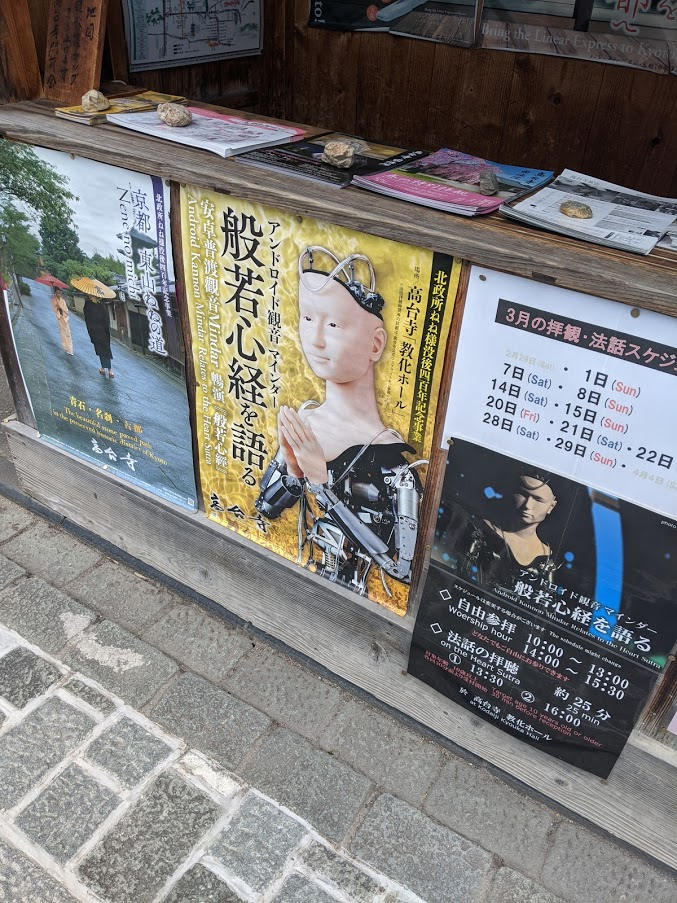
\includegraphics[scale=.55]{MVIMG_20200320_122141.jpg}
\end{center}

Absolutely nothing could go wrong with this.

\subsection{}
Why?

are we still here? Just to suffer? Every night, I can feel my leg... And my arm... even my fingers... The body I've lost... the comrades I've lost... won't stop hurting... It's like they're all still there. You feel it, too, don't you? I'm gonna make them give back our past!

or maybe you were looking for...

Science isn't about WHY. It's about WHY NOT. Why is so much of our science dangerous? Why not marry safe science if you love it so much. In fact, why not invent a special safety door that won't hit you on the butt on the way out, because you are fired.

Either way, the real "Why?" I'm asking is "Why do I have to use LaTeX? I spent an hour working on tables and they're still throwing errors that don't make any sense at all."

\pagebreak

\section{Lab Seven}

\subsection{}
Matt Smith: a great Doctor, or the greatest Doctor? Bonus: What about Jodie?

Matt Smith was the last of 3 extremely unique and interesting Doctors and is my personal favorite. Unfortunately, I fell out of watching \textit{Doctor Who} after him, so I don't have much comment on either Peter Capaldi or Jodie Foster. Of course, 9-11 were mainly what I watched, much like everyone else. Of those 3, I hold Eccleston's performance in very high regard, but he pales in comparison to how iconic Tenant made the character. All that said, Smith's mannerisms make him my favorite Doctor. The Doctor is an inherently strange person, never quite fitting in (not that he wants to). Eccleston and Tenant brought life and humanity to the character (well, as much as you can bring to a nonhuman), but Smith rolled all that in with an additional total weird-out factor. In addition, the stories he was featured in showed the Doctor indulging in a bit less blind action, focusing more on his curiosity. There's a reason why I'm more of a \textit{Next Generation} guy, and that more mystery focused storytelling was definitely playing on that. To me, he is definitely the greatest Doctor of them all.

I would also like to submit to the jury this picture of me at 16 in 11th grade just after a costume day at my high school:

\begin{center}
    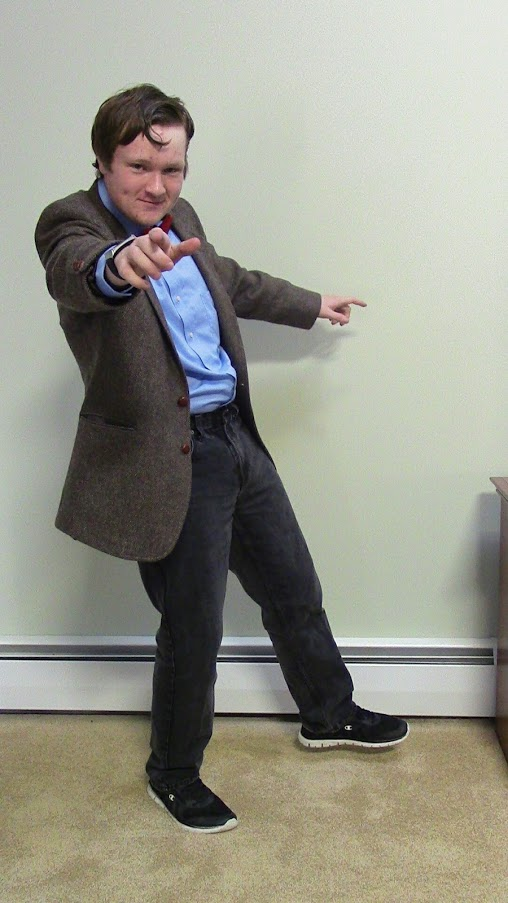
\includegraphics[scale=.35]{IMG_1895.jpg}
\end{center}

I unfortunately do not have a good picture of it right now, but I also own a full size, handmade replica of Tom Baker's scarf. I used to enjoy winter camping trips with the Scouts, so it was an excellent way to have a very heavy duty bit of winter gear while also looking nice.

\end{document}
